\chapter{Implementierung}\label{Implementierung}
Dieses Kapitel gibt eine Übersicht über den grundsätzlichen Aufbau des Programms und beleuchtet dann einige Aspekte und Probleme näher.
\section{Übersicht}
Die Klassen des Projektes lassen sich in die funktionalen Klassen im Hintergrund und die GUI-Klassen zur Darstellung und Interaktion mit dem User unterteilen. Das Projekt nutzt keine externen Pakete. Die Oberfläche ist aus Swing-Kompenenten gebaut. Das Projekt nutzt das Observer-Pattern. Nach Änderungen am Graphen o.ä. werden alle Observer benachrichtigt, welche alle darstellenden Komponenten sein sollten, die sich dann entsprechend aktualisieren können.

Ein grundsätzliches Problem bei der Implementierung ist, dass Java es nicht erlaubt, konstante Pointer benutzen, also ein Read-Only-Zugriff auf Objekte. Z.B. muss auf die Listen der Kanten und Knoten zum Zeichnen zugegriffen werden. Das bedeutet aber auch, dass durch diesen Zugriff die Objekte verändert werden könnten, was zu inkonsistenten Zuständen führen könnte (z.B. müssen die Kanten sowohl in die globale Liste, als auch die lokale Liste des Startzustandes eingetragen werden). Man könnte dies umgehen, indem man eine Wrapper-Klasse erstellt, die nur Getter-Methoden öffentlich zur Verfügung stellt. Das ist aber ein unverhältnismäßiger Aufwand.
\subsection{Funktionale Klassen}
\begin{figure}[htbp]
\centering
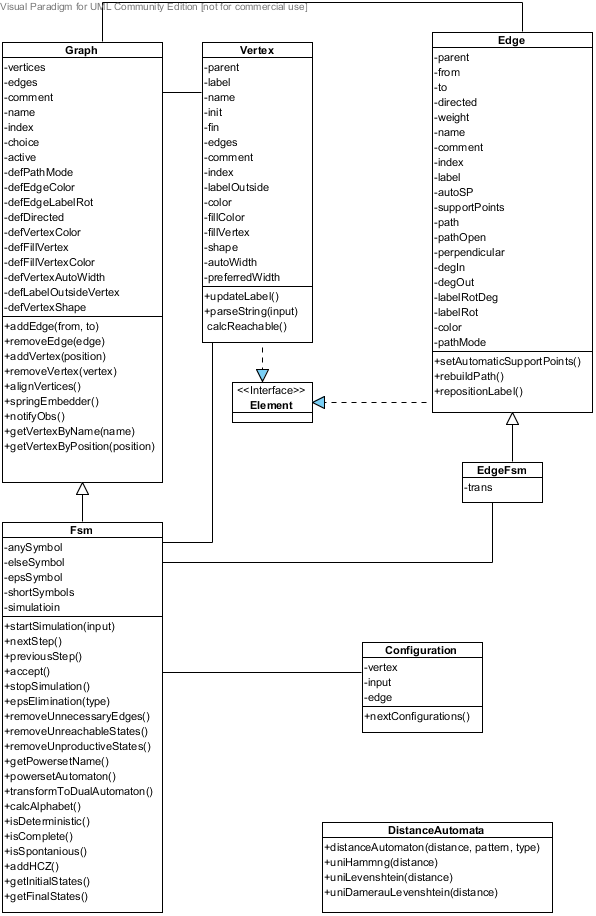
\includegraphics[width=\linewidth,height=\textheight,keepaspectratio]{pic/fsm}%
\caption{Klassendiagramm funktionale Klassen mit den wichtigsten Attributen und Methoden}%
\end{figure}
Die Hauptklasse ist die Klasse Graph, welche einen grundlegende Eigenschaften eines Graphen implementiert und die Knoten und Kanten hält.

Die Klasse Fsm erweitert die Klasse Graph um automatenspezifische Aspekte, das beinhaltet den Austausch der Kanten gegen eine für Automaten erweiterte Version, Methoden zur Simulation von Eingaben und die Algorithmen auf Automaten.

Knoten werden durch die Klasse Vertex repräsentiert, Kanten durch die Klasse Edge, bzw. EdgeFsm, welche die Kanten von Graphen um Übergänge erweitert. Diese Klassen implementieren das leere Interface Element, damit z.B. für eine Auswahl beide Klassen gleichartig gespeichert werden können.

Für die Simulation wird die Klasse Configuration benutzt. Sie repräsentiert einen Berechnungsschritt während der Simulation, also den aktuellen Zustand mit der Rest\-eingabe. Außerdem enthält die Klasse eine Funktion um eine Menge von Folgekonfigurationen zu berechnen.

Die Klasse DistanceAutomata enthält ausschließlich statische Methoden zur Erzeugung verschiedener Abstandsautomaten (universell und speziell).

\subsection{GUI-Klassen}
\begin{figure}[htbp]
\centering
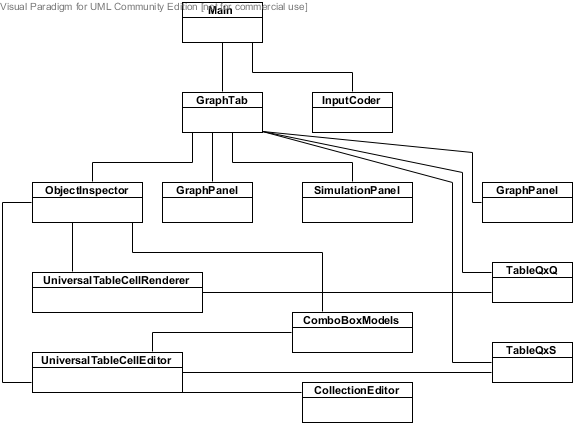
\includegraphics[width=\linewidth,height=\textheight,keepaspectratio]{pic/gui}%
\caption{Klassendiagramm GUI-Klassen ohne Attribute und Methoden}%
\end{figure}
Die Hauptklasse ist die Klasse Main. Sie ist ausführbar und erstellt ein JFrame mit einer Menüleiste und einer JTabbedPane. Hierin werden beliebig viele Automaten-/Grapheneinheiten repräsentiert durch die Klasse GraphTab. Hierin sind der Objektinspektor, die graphische Visualisierung, QxQ- und QxS-Tabelle und die Simulationssteuerung mit den entsprechenden Klassen Objectinspector, GraphPanel, TableQxQ, TableQxS und SimulationPanel angeordnet. Alle Tabellen (also QxQ, QxS und Objektinspektor) benutzen als Renderer zur Darstellung den UniversalTableCellRenderer und als Editor den UniversalTableCellEditor. Die Modelle, die den Tabellen die Daten liefern, sind Unterklassen der entsprechenden Komponente.

Die Klasse ComboBoxModels enthält Modelle und Renderer für ComboBoxen (mit Knoten oder mit Elementen).

Die Klasse CollectionEditor wird von dem UniversalCellEditor benutzt und zeigt ein Fenster zur Bearbeitung von Listen, Sets und Maps.

InputCoder ist ein Fenster, welches dazu da ist, die Eingabe für universelle Abstandsautomaten zu kodieren.

\section{parseString}
Bei den Beschriftungen von Knoten und Kanten ist Hoch- und Tiefstellen von Text möglich. Dafür sind zwei Implementierungen denkbar. Eine Möglichkeit wären Attributed Strings. Im folgenden Beispiel sind die Zahlen 5-7 hochgestellt.
\begin{lstlisting}
AttributedString as1 = new AttributedString("1234567890");
as1.addAttribute(TextAttribute.SUPERSCRIPT, TextAttribute.SUPERSCRIPT_SUPER, 5, 7);
g2d.drawString(as1.getIterator(), 15, 60);
\end{lstlisting}

Die Alternative beruht darauf, dass (fast) alle Swing-Komponenten HTML darstellen können. Das folgende Beispiel stellt ebenfalls die Zahlen 5-7 hoch. 
\begin{lstlisting}
label1.setText("<html>1234<sup>567</sup>890</html>");
\end{lstlisting}

Umgesetzt ist die zweite Methode. Beim setzten von Beschriftungen wird der String nach den formatierenden Symbolen (\_, \^\  und \textbackslash) gesucht und dann in entsprechenden HTML-Code umgesetzt. Dabei ist die Reihenfolge der Auswertung wichtig.
\begin{lstlisting}
		public static String parseString(String s) {
        StringBuilder t = new StringBuilder();
        Stack<String> open = new Stack<String>();
        boolean esc = false;
        boolean ins = false;
        boolean html = false;
        for (int i = 0; i < s.length(); i++) {
            final char c = s.charAt(i);
            if (esc) {
                t.append(c);
                esc = false;
                if (ins) {
                    t.append(open.pop());
                    ins = false;
                }
            } else if (c == '\\') {
                esc = true;
            } else if (ins && c != '{') {
                t.append(c).append(open.pop());
                ins = false;
            } else if (c == '_') {
                t.append("<sub>");
                open.add("</sub>");
                ins = true;
                html = true;
            } else if (c == '^') {
                t.append("<sup>");
                open.add("</sup>");
                ins = true;
                html = true;
            } else if (c == '{') {
                if (!ins) {
                    t.append(c);
                } else {
                    ins = false;
                }
            } else if (c == '}') {
                if (open.isEmpty()) {
                    t.append(c);
                } else {
                    t.append(open.pop());
                }
            } else {
                t.append(c);
            }
        }
        while (open.size() > 1) {
            t.append(open.pop());
        }
        if (ins) {
            if (open.pop().equals("</sub>")) {
                t.append('_');
            } else {
                t.append('^');
            }
        } else if (!open.isEmpty()) {
            t.append(open.pop());
        } else if (esc) {
            t.append('\\');
        }
        if (html) {
            t.append("</nobr></html>");
            t.insert(0, "<html><nobr>");
        }
        return t.toString();
    }
\end{lstlisting}
\section{Tabellen}
Tabellen in Java sind etwas gewöhnungsbedurftig, aber dafür recht mächtig. Es gibt drei Teile, über die man sich beim Bau einer Tabelle Gedanken machen muss.

Das erste ist das TableModel. Die wichtigen Methoden in dieser Klasse sind \lstinline[breaklines=true]{getValueAt(int rowIndex, int colIndex)} und für editierbare Tabellen \lstinline[breaklines=true]{isCellEditable(int rowIndex, int colIndex)} und \lstinline[breaklines=true]{setValueAt(Object value, int rowIndex, int columnIndex)}. Es gibt vorgefertigte einfache TableModels, die aber schnell an die Grenzen stoßen. Alle Table\-Mo\-dels (Objektinspektor, $Q \times Q$-Tabelle und $Q \times S$-Tabelle) sind überschrieben und geben in Abhängigkeit der Position direkt Daten des Graphen bzw. Automaten weiter bzw. schreiben diese Werte. Für Werte bei denen eine Referenz übergeben wurde und nur dieses Objekt bearbeitet und nicht überschrieben wurde (z.B. Listen) muss die setValueAt-Methode gar nichts unternehmen.

Der Renderer ist für die Darstellung verantwortlich. Der Defaultrenderer ist nur geeignet, wenn eine gesamte Spalte einen eindeutigen Typ hat. Dann kann er z.B. Boolean-Werte durch eine CheckBox darstellen. Objects werden einfach durch ihre Stringrepräsentation dargestellt. Alle Tabellen benutzen den UniversalTableCellRenderer, welcher die Methode \lstinline{public Component getTableCellRendererComponent(JTable table, Object value, boolean isSelected, boolean hasFocus, int row, int column)} überschreibt. In Abhängigkeit des Types von value (Test mit instanceof) wird eine geeignete Darstellung in einem JLabel erstellt und zurückgegeben.

Der Editor übernimmt die Bearbeitung der Werte. Zum einen muss die Methode \lstinline{public Component getTableCellEditorComponent(JTable table, Object value, boolean isSelected, int rowIndex, int colIndex)} überschrieben werden, welche -- wie beim Renderer -- abhängig vom Typ von value eine geeignete Komponente zur Bearbeitung des Wertes zurückliefert. Als zweites muss die Methode \lstinline{public Object getCellEditorValue()}, welche nach dem Beenden des Editierens aufgerufen wird und den neuen Wert an das TableModel zurück gibt, überschrieben werden. Dafür wird beim Wählen der Komponente diese gespeichert, damit dann daraus der Wert (mit dem richtigen Typ) zurückgegeben werden kann.

Ein Schwierigkeit bei der Implementierung war, dass das Beenden des Editierens einer Zelle nur durch explizite Aufforderung durch den Benutzer geschieht, also durch Auswahl einer anderen Zelle mit der Maus oder Bestätigen durch Enter oder Tab. Zum einen werden dadurch die neuen Werte erst spät übernommen, zum anderen kann es zu Problemen kommen, wenn sich während des Editierens der Inhalt der Zelle ändert, oder gar der Typ (z.B. wenn beim Objektinspektor ein anderer Elementtyp (Graph, Knoten, Kante) ausgewählt wird). Es soll eine Möglichkeit geben mit \lstinline{table.putClientProperty("terminateEditOnFocusLost", Boolean.TRUE);} das Editieren automatisch zu stoppen, aber das hat nicht funktioniert. Es funktioniert ebenfalls nicht, das Editieren zu Stoppen, wenn die Tabelle den Focus verliert, da die Tabelle den Focus auch nicht hat, wenn der Editor in der Tabelle ihn hat. Also muss jeder Editor einen FocusListener bekommen, in dem das Editieren bei FocusLost explizit gestoppt werden kann. Dabei ist zu beachten, dass z.B. JSpinner keinen Focus haben, sondern nur das TextFeld des Editors des Spinners, außerdem sollte dem TextFeld Focus gegeben werden, wenn direkt ein Button des Spinners benutzt wird. Weiterhin ist darauf zu achten, nicht bei jedem Focus-Verlust das Editieren zu beenden, denn wenn eine andere Zelle ausgewählt wird, wird das Editieren erst gestoppt und der nächste Editor erhält den Focus danach, d.h. es würde das Editieren sofort nocheinmal gestoppt werden. Ähnliches gilt, wenn der Editor aus mehreren Komponenten besteht (z.B. Punkte mit zwei Spinners). Die Probleme wurden gelöst, indem alle Editorkomponenten, die einen Focus erhalten können, in einer Liste gespeichert werden und beim FocusLost getestet wird, ob die neue Komponente mit dem Focus nicht in dieser Liste ist.

Weiterhin ist zu beachten, dass beim Stoppen des Editierens nicht automatisch die neuen Werte beim JSpinner gesetzt werden, es sollte also vor dem Abfragen der Werte ein \lstinline{((JSpinner.DefaultEditor) spinner.getEditor()).commitEdit()} aufgerufen werden. Bei Werten die über ein eigenes Fenster (Collection-Editor, Color) und bei Boolean-Werten sollte das Editieren automatisch sofort nach dem Zurückgeben der Komponente gestoppt werden, damit die Änderungen übernommen werden können. Das funktioniert, indem unmittelbar nach der Auswahl der Komponente, der stopEditing-Befehl in die Java-EventQueue eingetragen wird:
\begin{lstlisting}
java.awt.EventQueue.invokeLater(new Runnable() {
	@Override
	public void run() {
		stopCellEditing();
	}
});
\end{lstlisting}
Eine ComboBox sollte über einen ActionListener nach der Auswahl eines Wertes das Editieren beenden.\\
Außerdem wird für alle textuellen Editoren ein Timer gestartet, der nach 3 Sekunden ohne Eingabe das Editiern automatisch beendet (durch Key- und MouseListener wird dieser Timer bei beliebiger Interaktion neu gestartet).

\begin{table}
\begin{sloppypar}\noindent \begin{longtable}{p{(\textwidth-12\tabcolsep-12\fboxrule)/6}|p{(\textwidth-12\tabcolsep-12\fboxrule)/6+3pt}|p{(\textwidth-12\tabcolsep-12\fboxrule)/6-3pt}|p{(\textwidth-12\tabcolsep-12\fboxrule)/6}|p{(\textwidth-12\tabcolsep-12\fboxrule)/6}|p{(\textwidth-12\tabcolsep-12\fboxrule)/6}}
 \textbf{Typ}&\textbf{Werte}&\textbf{Renderer}&\textbf{Editor}&\textbf{Stop Editing}&\textbf{Listener}\\
 \hline\hline
 \endhead
String & Name, Kommentar & String & JTextField & Focus,\newline Timer & Focus,\newline Key, Mouse \\ \hline
Character & Automaten-Symbole & toString & JTextField mit DocumentFilter & Focus,\newline Timer & Focus, Key, Mouse \\\hline
Color & Farben & Label-Farbe, String, RGB-Wert & JColor\-Chooser & instantan & - \\\hline
Boolean & Initial, Final, Füllen, autom. Breite usw. & Haken/\newline Kreuz & JLabel & instantan & - \\\hline
Integer & Index, Breite, Höhe & toString & JSpinner & Focus,\newline Timer & (Focus,\newline Key,\newline Mouse,)\newline Change \\\hline
Double & Winkel, Gewicht & toString & JSpinner & Focus,\newline Timer & (Focus, Key,\newline Mouse,)\newline Change \\\hline
Point & Positionen & int, int & 2 JSpinner & Focus,\newline Timer & je (Focus, Key,\newline Mouse,)\newline Change \\\hline
Shape & Form & enum (String) & JCombo\-Box & Focus,\newline Auswahl & Focus,\newline Action \\\hline
PathMode & Ecken abrunden & enum (String) & JCombo\-Box & Focus,\newline Auswahl & Focus,\newline Action \\\hline
Vertex & Start, Ziel & getName() & JCombo\-Box & Focus,\newline Auswahl & Focus,\newline Action \\\hline
List & Hilfspunkte, QxS-Eintrag & zeilenweise & Collection\-Editor & instantan & - \\\hline
Set & Übergänge & zeilenweise & Collection\-Editor & instantan & - \\\hline
Map & Symbol\-abkürzungen & zeilenweise \newline Key $=>$ Val & Collection\-Editor & instantan & - \\\hline
\end{longtable}\end{sloppypar}
\caption{Übersicht über Typen und dazugehörige Editoren}
\end{table}
\section{Shapes}
Für die graphische Repräsentation der Knoten und Kanten werden Klassen, die das Interface Shape implementieren, benutzt. Knoten können beliebige RectangularShape annehmen; Arc2D, Ellipse2D, Rectangle2D und RoundRectangle2D werden von Java mitgeliefert. Bis auf Arc2D können diese Formen auch als Knotenform im Objektinspektor ausgewählt werden. Es wäre ohne weiteres möglich, eine Klasse zu schreiben, die RectangularShape implementiert und diese dann als Knotenform zu benutzen. Die Shape-Klassen lassen sich dann sehr leicht auf den graphischen Kontext eines Panels zeichnen. Mit der contains-Methode lässt sich überprüfen, ob z.B. ein Mausklick innerhalb eines Shapes gemacht wurde.

Kanten werden als Path2D repräsentiert. Dieser setzt sich aus Abschnitten von geraden Linien, quadratischen oder kubischen Bezierkurven zusammensetzen. Der Pfad wird vom Startknoten zum Zielknoten über die Hilfspunkte berechnet. Berechnung von Start und Zielpunkt erfordert etwas Rechnerei, weil es nicht ausreicht, vom Zentrum oder Rand der BoundingBox die Linie zu zeichnen, dadurch würde ein Teil der Linie innerhalb des Knotens liegen (was zum einen bei Transparenz ein Problem ist, zum anderen den Pfeil verschwinden lässt) oder die Linie in der Luft schwebt. Zunächst wird die Richtung bestimmt als Vektor zwischen Start bzw. Ziel und wenn vorhanden nächster Hilfspunkt oder Ziel bzw. Start berechnet. An diesem Vektor wird dann so lange \glqq entlang gelaufen\grqq, bis man gerade innerhalb des Knotens bzw. gerade außerhalb des Knotens ist (Überprüfung mit contains()).

Ohne Abrunden von Ecken wird einfach eine Linie von Hilfspunkt zu Hilfspunkt gezeichnet. Mit Abrundung werden Bezierkurven von dem Mittelpunkt der Verbindung letzter Hilfspunkt (bzw. Start) zum nächsten Hilfspunkt (bzw. Ziel) mit dem aktuellen Hilfspunkt als Stützpunkt gezeichnet. Bei starker Abrundung wird eine quadratische Bezierkurve benutzt. Bei leichter Abrundung wird eine kubische Bezierkurve mit dem aktuellen Hilfspunkt für beide Stützpunkte benutzt, wodurch der Hilfspunkt stärker gewichtet wird. Die fehlenden Enden werden durch einfache Linien ergänzt.

Die Auswahl der Pfade erfolgt mit der intersect-Methode und einem um den gewünschten Punkt gelegtem Kreis. Dabei ist es ärgerlich, dass Java den Pfad automatisch schließt -- grundsätzlich durch eine direkte Verbindung von Start und Ziel. Das ist unproblematisch ohne Hilfspunkte, aber mit Hilfspunkten entstehen dadurch unerwünschte Formen mit einem echten Flächeninhalt. Um dies zu umgehen, muss der Pfad nocheinmal komplett rückwärts berechnet werden. Es werden also zwei Pfade für eine Kante gehalten, einmal der einfache zum Zeichnen und ein weiterer geschlossener zur Überprüfung eines Schnittes. Die Punkte des Pfeiles müssen extra berechnet werden unter Berücksichtigung der entsprechenden Winkel.

Die Beschriftungen sind in JLabels gespeichert. Es hat sich herausgestellt, dass man es vermeiden sollte, die Labels dem Container hinzuzufügen, da dadurch durchgehend repaints aufgerufen wurden. Stattdessen sollte man die Labels mit der paint-Methode in den graphischen Kontext des Panels zeichnen. Das bedeutet, dass man keine Mouse-Listener auf den Labels verwenden kann, sondern in dem MouseListener des Panels über contains überprüft werden muss, ob der Mausklick im Label war. Gleichzeitig wird es dadurch sehr einfach, das Label zu drehen, indem man vor dem Zeichnen den graphischen Kontext dreht. Diese Drehung muss auch bei der contains-Überprüfung beachtet werden.
\section{Defaultwerte}
Zunächst waren die Default-Werte als statische Klassenattribute direkt in der Kante bzw. dem Knoten gespeichert. Das hat den großen Nachteil, dass bei mehreren geöffneten Automaten bzw. Graphen die Defaultwerte global für alle gelten. Außerdem werden dadurch die Defaultwerte nicht mitgespeichert.

Die Alternative war, die Defaultwerte im Graphen (Automaten) zu speichern und in den Knoten-/Kantenobjekten das Elternelement zu speichern, damit auf diese Werte zugegriffen werden kann.

Ein weiterer Aspekt war, dass zunächst ein boolean-Attribut inherit benutzt wurde, welches angegeben hat, ob die Kante bzw. der Knoten die Standardeinstellungen erben soll. In diesem Fall wurde direkt der Standardwert im Getter zurückgegeben. Bei der Änderung eines solchen Wertes wurde auf inherit auf false gesetzt. Diese Art des inherit-Flags hatte den Vorteil, dass, wenn der Standard-Wert geändert wurde, dieser sofort automatisch von den Knoten bzw. Kanten übernommen wurde. Auf der anderen Seite entstanden dadurch unschöne Effekte, dass sich  mit dem Ändern des inherit-Flags mehr Eigenschaften änderten, als eigentlich der Fall sein sollte. Deshalb wurde das Flag entfernt und stattdessen gibt es eine Methode, um die Werte zurück auf die Defaultwerte zu setzen. Nun werden Änderungen der Defaultwerte selbst nicht rückwirkend übernommen und gelten nur für neue Kanten und Knoten. Es wäre aber denkbar, dafür eine Option einzubauen, die dafür sorgt, dass der Defaultwert auch bei bereits vorhandenen Elementen gesetzt wird.
\section{Graph/Fsm-Erweiterung}
Da die Automaten eine graphische Darstellung unterstützen sollen, können Automaten als Graphen mit zusätzlichen Eigenschaften, die speziell für Automaten benötigt werden, betrachtet werden. Es bietet sich daher an, zunächst eine Klasse Graph zu erstellen, die alle Informationen für eine graphische Darstellung mit Knoten und Kanten enthält und diese dann um die zusätzlichen Funktionen zu erweitern. Das bietet die Möglichkeit, im Programm auch Graphen ohne Automateneigenschaften zu konstruieren. Lediglich zwei Eigenschaften von Graphen haben für Automaten keine Bedeutung, nämlich Kantengewichte, welche aber nicht stören, und die Möglichkeit ungerichtete Kanten zu benutzen. Das wird im Automaten durch ein Überschreiben der Setter-Methode für diesen Wert erreicht.

Beim Erweitern des Graphen müssten auch die Klassen Edge und Vertex erweitert werden, da die wesentlichen Eigenschaften der Automaten in diesen Klassen liegen. Kanten benötigen zusätzlich die Übergangsrelation und Knoten die Eigenschaften Start- bzw. Finalzustand. (Für die Potenzmengenkonstruktion haben die Knoten auch noch Felder und Methoden zur Berechnung der erreichbaren Zustände). Die Klasse Edge wurde auch tatsächlich mit EdgeFsm um die Übergangsrelation erweitert. Nachteil davon ist, dass auch z.B. Methoden zum Hinzufügen im Automaten durch die andere Klasse überschrieben werden müssen. Auch erfordert dies öfters Casts, wenn zunächst nur die allgemeine Kantenklasse vorliegt und die Automateneigenschaften benötigt werden. Wegen dieser Unbequemlichkeiten wurde bei den Knoten zunächst darauf verzichtet, diese zu erweitern, sondern die benötigten Felder und Methoden liegen in der allgemeinen Knotenklasse Vertex, da diese Graphen nicht stören. Der Sauberkeit halber sollte eine Trennung in Vertex- und VertexFsm-Klasse nachgeholt werden.
\section{Simulation}
Zunächst war die Simulation so implementiert, dass in einer Liste die aktiven Zustände (und zur Darstellung aktive Kanten) gespeichert wurden und global der Resteingabe-String. Bei der Berechnung des nächsten Schrittes wurde von jedem aktiven Zustand die Erreichbarkeit mit der Resteingabe überprüft und die Resteingabe entsprechend angepasst. Die neuen aktiven Elemente waren dann die benutzen Kanten mit ihren Zielzuständen. Spontan erreichbare Zustände wurden nach jedem Berechnungsschritt hinzugefügt. Das funktioniert einfach und gut, solange die Blocklänge konstant ist und keine spezielle Berechnung nachvollzogen werden soll, denn dafür werden mehr Informationen gebraucht, bzw. unterschiedliche Berechnungen können eine unterschiedliche Resteingabe haben.

Jetzt hält die Simulation eine Liste von Berechnungen, was einer Liste einer Liste von Konfigurationen entspricht, wobei eine Konfiguration ein aktiver Zustand mit der dazugehörigen Resteingabe ist. Eine Konfiguration wird durch die Klasse Configuration repräsentiert. Zusätzlich kann zur Visualisierung die aktive Kante gespeichert werden. Die Klasse Configuration bietet eine Methode, um eine Liste von Folgekonfiguration zu berechnen. Spontane Übergänge erfolgen nun wie andere Übergänge auch in einem eigenen Simulaitonsschritt. Die Liste der aktiven Elemente wird weiterhin für die Visualisierung genutzt und muss entsprechend nach einem Berechnungsschritt aus der Konfiguration berechnet werden.

Bei der Berechnung der Folgekonfigurationen wird jeder von dem Zustand der Konfiguration aus mögliche Übergang mit dem Beginn der Resteingabe gleicher Länge verglichen. Dabei gibt es einige Besonderheiten. Any-Übergänge funktionieren immer. Spontane Übergänge auch, verbrauchen aber keinen Buchstaben und müssen für Else-Übergänge gezählt werden. Else-Übergänge müssen zunächst gemerkt werden, diese werden nur den Übergängen hinzugefügt, wenn nur spontane gemacht wurden (deshalb müssen sie gezählt werden). Tritt keiner dieser Sonderfälle auf, wird der Block (auch Länge 1) zeichenweise verglichen. Dabei müssen die Abkürzungssymbole umgesetzt werden.

Der Start der Simulation erfolgt mit der Methode startSimulation(String input). Beim Start der Simulation werden Konfigurationen mit der vollen Eingaben für jeden Startzustand in die Liste eingetragen. Der nächste Simulationsschritt wird mit der Methode nextStep() berechnet. Dabei wird für jede letzte Konfiguration der Berechnung in der Liste der Berechnungen die Folgekonfigurationen berechnet. Die alte Berechnung wird aus der Liste entfernt und für jede Folgekonfiguration wird die alte Berechnung konkateniert mit der entsprechenden Folgekonfiguration wieder hinzugefügt. Dabei muss explizit der Fall ausgeschlossen werden, dass ein spontaner Kreis geschlossen wird, was nicht zur Erkennung der Sprache beiträgt, aber unendlich lange Berechnungen produziert. Dafür wird für jede Konfiguration mit gleichem Input überprüft, ob bereits eine Konfiguration mit dem gleichen Zustand existiert.
\section{Algorithmen}
\subsection{Automaten optimieren}
Zu dieser Kategorie zählen Entfernen von unproduktiven Zuständen, Entfernen von unerreichbaren Zuständen, Entfernen unnötiger und zusammenfassen mehrfacher Kanten und das Hinzufügen eines Hotel-California-Zustanden. All dies sind wenig komplexe Algorithmen.

Für das Auffinden von unerreichbaren Zuständen wird von den Startzuständen aus eine Breitensuche durchgeführt, für das Auffinden von unproduktiven Zuständen wird dies im dualen Automaten gemacht. Dabei werden die erreichbaren Zustände durch die Startzustände initialisiert. Zu diesen Zuständen wird sich gemerkt, ob sie schon verarbeitet wurden. Für alle erreichbaren, aber nicht verarbeiteten Zustände, werden die Nachbaren zu den erreichbaren Zuständen hinzugefügt, anschließend wird dieser Zuständ als verarbeitet markiert. Wenn keine Änderungen mehr auftreten, also alle erreichbaren Zustände verarbeitet wurden, sind alle erreichbaren Zustände gefunden und die übrigen können entfernt werden.

Für die Optimierung der Kanten wird durch alle Kanten iteriert. Ist die Übergangsmenge leer, wird die Kante entfernt. Andernfalls wird überprüft, ob bereits eine Kante mit den selben Start- und Zielzuständen gefunden wurde. Ist dies der Fall, werden alle Übergänge den Übergängen der anderen Kante hinzugefügt und diese Kante entfernt.

Das Hinzufügen eines HCZ kann intelligent oder nicht intelligent geschehen. Bei der nicht intelligenten Form wird einfach ein Zustand, welcher weder Start- noch Endzustand ist, ergänzt und von jedem Zustand aus wird ein Else-Übergang zu diesen Zustand hinzugefügt. Bei der intelligenten Version muss zunächst das Alphabet berechnet werden. Dann werden nur dann Übergänge mit den verbliebenden Zeichen hinzugefügt, wenn der Zustand lokal nicht vollständig ist. Wie bei der globalen Vollständigkeit, ist die Überprüfung auf lokale Vollständigkeit bei variabler Blocklänge sehr schwierig. Außerdem könnte überprüft werden, ob bereits ein HCZ existiert und dieser benutzt werden. Die intelligente Variante ist noch nicht implementiert.
\subsection{Dualer Automat}
Die Berechnung des dualen Automaten ist sehr einfach. Zunächst wird durch alle Zustände iteriert. Ist ein Zustand Startzustand, wird er Endzustand und umgekehrt. Anschließend wird durch alle Kanten iteriert und Start- mit Zielknoten vertauscht.
\subsection{Epsilon-Elimination}
Die Elimination spontaner Übergänge kann durch Absorbtion von links, rechts oder beidseitig erfolgen. Bei der Absorbtion von links werden erst spontane Übergänge gemacht und dann der normale Übergang angehängt, von rechts erst normaler Übergang und dann spontane Übergänge und beidseitig werden vorher und nacher spontane Übergänge gemacht.

Es wird also von jedem Zustand n aus bei nicht rechts die Epsilon-Erreichbarkeit berechnet, sonst ist nur n erreichbar. Nun wird vom Zustand n für jede Kante e eine Kante mit dem Übergang von n zum Zielknoten von e hinzugefügt. Bei nicht links außerdem zu den vom Zielknoten von e durch spontane Übergänge erreichbaren Zuständen. Es spielt keine Rolle, ob dabei spontane Kanten kopiert wurden. Die neuen Kanten müssen gespeichert werden, da die neuen Kanten im vorigen Schritt nicht benutzt werden dürfen. Erst am Ende werden die spontanen Übergänge selbst entfernt.
\subsection{Potenzmengenkonstruktion}
Durch die Sonderfunktionen bei der Berechnung ist die Potenzmengenkonstruktion sehr aufwändig.

Zunächst muss von jedem Knoten die Erreichbarkeit (ohne spontane Übergänge) berechnet werden. Diese wird in einer Map gespeichert, die von Übergangslabeln auf eine Menge von Zuständen abbildet. Dabei wird jeder mögliche Übergang betrachtet, wobei Any und Else-Übergänge nicht gesondert betrachtet werden und spontane Übergänge übersprungen werden. Der durch den Übergang erreichbare Zustand sei n. Existiert dieser Übergang in der Map, wird n der dazugehörigen Zustandsmenge hinzugefügt. Existiert er nicht, muss überprüft werden, ob es eine Überschneidung von diesem Übergang mit einem Übergang in der Map gibt, was durch die abkürzenden Symbole vorkommen kann. Gibt es eine Überschneidung, müssen dieser Eintrag entfernt und bis zu drei neue Einträge hinzugefügt werden: ein Eintrag, mit dem Übergangslabel, das übrig bleibt, wenn man die Überschneidung von dem ursprünglichen Übergang abzieht, und der ursprünglichen Zustandsmenge, ein Eintrag mit der Überschneidung und der ursprünglichen Zustandsmenge erweitert um n und ein Eintrag mit dem Übergangslabel, das übrig bleibt, wenn man die Überschneidung vom aktuellen Übergang abzieht, und n. Gibt es keine Überschneidung wird ein neuer Eintrag mit dem aktuellen Übergang und n angelegt.

%intersection berechnen
Um die Überschneidung zu berechnen, werden beide Übergänge zeichenweise verglichen. Stimmen die Zeichen überein (auch bei Symbolabkürzungen), ist dies ein Teil der (potentiellen) Überschneidung. Ist dies nicht der Fall, müssen beide Zeichen auf Symbolabkürzungen überprüft und ggf. miteinander verglichen werden. Finden sich dabei keine gleichen Zeichen, gibt es keine Überschneidung. Beim Vergleich ist es möglich, dass mehrere Zeichen gleich sind und so mehrere Überschneidungen entstehen. %TODO gedanken über präfixe, ich glaube das stimmt so nicht, wie es gerade ist.

%remaining berechnen
Um die Reste zu berechnen, wird für jedes Symbol des ersten Strings die entsprechende Menge von Zeichen angelegt, wobei die Zeichen des zweiten Strings jeweils abgezogen werden. Jedes in den den Mengen verbliebende Zeichen wird dann einmal an entsprechender Stelle im ersten Originalstring eingesetzt und der Menge der Reste hinzugefügt.

Bei der eigentlichen Potenzmengenkonstruktion wird mit dem Metazustand, der aus der Menge der Startzustände besteht gestartet. Für diesen und jeden weiteren entstandenen Metazustand wird folgendes getan. Die Übergänge aller Zustände der Zustandsmenge des Metazustandes werden zusammengefasst und zwar auf die gleiche Art wie bei der Berechnung der Erreichbarkeit von einem Knoten aus. Bei dieser Gelegenheit werden gleich leere Else-Übergänge entfernt, also wenn es zu dem Else-Übergang noch ein Any-Übergang beim gleichen Knoten gibt. Anschließend müssen Any- und Else-Übergänge gesondert behandelt werden. Die Zustände, die über das Any-Symbol erreichbar sind, müssen jedem Übergang hinzugefügt werden. Die Zustände, die über das Else-Symbol erreichbar sind, müssen jedem Übergang der anderen Knoten hinzugefügt werden. Any-Symbole werden anschließend zu Else-Symbolen. Nun werden entsprechend der berechneten Übergänge Kanten und - sofern sie noch nicht existieren - neue Metazustände angelegt.
\begin{figure}[!htbp]
\centering
\subfloat[Any: Der zusammengesetzte Automat links wird zum Potenzmengenautomat rechts. Der Else-Übergang zu q$_6$ entfällt. Die Ziele der Any-Übergänge müssen sowohl den Zielen von 1 also auch den Zielen von 0 hinzugefügt werden. Damit kann der Any-Übergang dann zum Else-Übergang werden, um Determinismus zu gewährleisten.]{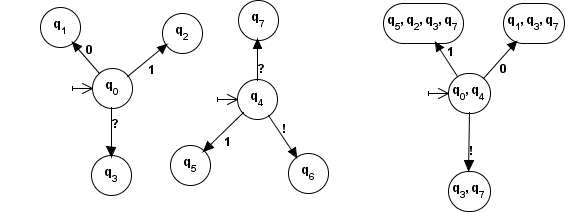
\includegraphics[scale=0.7]{pic/automata/beispielPMAany}}%
\hspace{0.1cm}
\subfloat[Else: Der zusammengesetzte Automat links wird zum Potenzmengenautomat rechts. Die Else-Übergänge werden jeweils nur den Übergängszielen der Übergangslabels des anderen Teilautomaten hinzugefügt.]{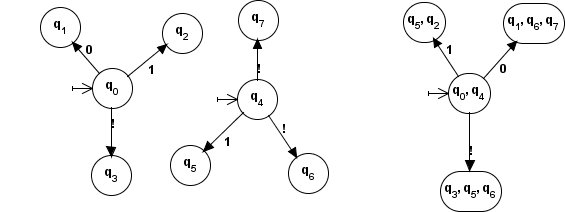
\includegraphics[scale=0.7]{pic/automata/beispielPMAelse}}%
\caption{Beispiele Potenzmengenkonstruktion Any und Else-Übergänge}%
\end{figure}

\subsection{Automateneigenschaften}
Vollständigkeit: Um die Vollständigkeit zu überprüfen, muss zunächst das Alphabet berechnet werden. Für variable Blockgrößen ist schwer feststellbar, ob der Automat vollständig ist. Bei konstanter Blockgröße größer als 1, ist zu entscheiden, ob ein Automat als vollständig gelten kann, da in dem Fall die Eingabe ein Vielfaches der Blockgröße sein muss, damit der letzte Schritt funktionieren kann. Grundidee ist für Automaten ohne Blöcke zu kontrollieren, ob für jedes Zeichen des Alphabetes ein Übergang existiert.\\
\textit{Hinweis: Die Funktion ist für Blöcke nicht vollständig implementiert.}

Determinismus: Beachte die hier benutzte Definition von Determinismus (\ref{Determinismus}). Bei der Überprüfung, ob der Automat deterministisch ist, muss überprüft werden, ob von einem Zustand bzw. der Epsilon-Erreichbarkeit ein Übergäng Präfix eines anderen ist (also evt. auch gleich ist).\\
\textit{Hinweis: Die Funktion ist für Blöcke nicht vollständig implementiert.}

Alphabet: Die Berechnung des Alphabetes erfolgt, indem jeder Übergang betrachtet wird und eine Liste der benutzten Zeichen erstellt wird. Blöcke werden dabei in ihre einzelnen Zeichen zerlegt. Any-, Else- und spontane Symbole werden dabei nicht berücksichtigt. Symbolabkürzungen werden umgesetzt.

Spontanität: Die Überprüfung, ob der Automat spontane Symbole benutzt, erfolgt durch ein Durchsuchen sämtlicher Übergänge nach dem spontanen Symbol.

Initial- bzw Finalzustande: Für die Rückgabe der Initial- bzw Finalzustande werden alle Zustände durchlaufen und ein Zustand der Liste hinzugefügt, wenn er entsprechend Initial- oder Finalzustand ist.
%\subsection{Kleene-Algorithmus}
%\subsection{Minimierung}
\endinput
